% Document Type: LaTeX
% Master File: ps5-merger.tex

\input ../6001mac.tex	% On ALTDORF.AI.MIT.EDU
\input psfig

\def\fbox#1{%
  \vtop{\vbox{\hrule%
     \hbox{\vrule\kern3pt%
 \vtop{\vbox{\kern3pt#1}\kern3pt}%
 \kern3pt\vrule}}% 
 \hrule}}

\begin{document}

\psetheader{Fall Semester, 1991}{Problem Set 5}

Issued: Tuesday, October 8

Tutorial preparation: see below

Written solutions due: Friday, October 18, in Recitation


Reading assignment: Finish Chapter 2, Section 3.1.

\bigskip

{\bf Quiz Announcement:}  Remember that Quiz 1 is on Wednesday, October
23.  The quiz 
will be held in Walker Memorial gymnasium (50-340) from 5--7PM or
7--9PM.  You may take the quiz during either one of these two periods,
but students taking the quiz during the first period will not be allowed
to leave the room until the end of the period.  The quiz is {\bf
partially} open book, meaning that you may bring a copy of the Scheme
manual, plus {\bf one} sheet of 8.5 by 11 inch paper, on which you may
place any crib notes you think will be useful.  The quiz will cover
material from the beginning of the semester through the material
presented in recitation on October 11, and through section 3.2
of the textbook.  

\section{Part 1. Tutorial exercises}

Due to the Columbus Day holiday and the upcoming quiz, this problem
set does {\em not} have any tutorial exercises.  The only required work is
in the lab assignment below. 
Please use the extra time to prepare for the quiz.


\section{Part 2. Laboratory Assignment: Merger Mania}

This assignment asks you to integrate three different file systems
using dispatch-by-type and data-directed programming techniques.
You should read section 2.3 of the book before doing this assignment.
In addition, the structure of one of the file systems is very
similar to a Huffman-coding-tree, which is described in detail in
section~2.2.6 of the book.  You should refer to that section if
you do not understand it from reading the code we give you in the
appendix.

\bigskip

\fbox{\hbox{\vbox{REMINDER: Whenever you are asked to write or complete some
implementation, you should not only turn in a listing of your code,
you should {\bf always} turn in a printout of an interactive {\sc Scheme}
session as an example of testing your code. Failure to explicitly test your
procedures will likely impair your grade on homework assignments which could,
in turn, impact your grade in the course.  It is always better
to openly admit that something doesn't work and where you think the bug(s) may
be (and even what you might do to try to fix them) than to imply that you
incorrectly think everything works by not showing any failing test cases.}}}

\section{An adaptation of a True Story of Our Time}

Recent chronic economic depressions have had significant impact upon the
computer industry.  Many small and medium-sized companies (and some biggies!!)
are being forced to merge to form conglomerates\footnote{Take 14.01 to learn more
about these economics buzz words.} in order to survive the high cost of
business
operation.  Among these unfortunate souls are three computer companies that
have decided to merge to form one single company.  They are {\bf Quince}, {\bf
Big Aquamarine} and {\bf Helios}.  These three companies are, however, very
worried about integrating their personnel files.  Their file systems are
structured differently, and they have so many employees that designing a
completely new file system would require them to hire 10 data entry clerks for
3 years to enter all the data into the new system.  The CEO at Quince, Al
Cheapo, thinks that this is too expensive.  He has appointed you to think up a
way of integrating the three file systems without having to modify the
internals of any one system.  You, of course, know a good trick for doing this,
if you have gone to the recent lectures.

\section{Problem 1}

Just when you were ready to begin work, a small fire broke
out in the computer lab at Quince.  The procedures for looking
up, inserting, and deleting employee records for Quince's
personnel file were destroyed from magnetic tapes as well as from
computer memory.  Your first task is to reconstruct those
procedures.  You begin by analyzing the
structure of Quince's personnel file, which looks like the diagram
shown in Figure~\ref{fig:box-n-ptr} (verify it in your mind!).

\begin{figure}[hbt]
\begin{center}
\mbox{\psfig{file=ps5-merger-fig1.ps}}
\end{center}
\caption{Box and pointer diagram of Quince's personnel file}\label{fig:box-n-ptr}
\end{figure}

Notice that the names of the employees are alphabetized from
left to right.  In fact, the personnel file is structured
exactly the same as Big Aquamarine's file structure, except
for one difference: the employees are alphabetically
arranged in Quince's file, while the employees
are randomly arranged in Big Aquamarine's file structure.
Reconstruct the {\tt lookup}, {\tt insert} and {\tt delete} procedures for
Quince's personnel file.  Try to make your procedures
efficient by using the fact that employee names are alphabetized.
Name these procedures {\tt lookup-ordered}, {\tt insert-ordered} and
{\tt delete-ordered}.

For your definition of {\tt insert-ordered}, you should find it convenient to
define a new procedure {\tt append-ordered} which takes two arguments: (1) a
{\tt pair} whose {\tt car} is a {\tt symbol}, and (2) a {\tt
sorted-list-of-pairs} where each pair's {\tt car} is a symbol and the pairs are
arranged such that their {\tt car}s are in alphabetical order from left to
right.  It should return a new list of pairs which looks like the old {\tt
list-of-pairs} but with {\tt pair} copied in so that all the pairs {\tt car}s
are in alphabetical order, including the newly added {\tt pair}.

Test each procedure using the miniaturized file
system provided in the appendix.
When you test out the {\tt insert-ordered}
procedure, use the given constructor {\tt make-record-table} to make a
new record with salary information for Alyssa, who makes 70~thousand
dollars a year at Quince.

Hand in a listing of your procedures and a {\sc Scheme} transcript of
a sample execution of each procedure.

Notice one peculiarity of the way we have defined our system:
if you insert a new record (e.g.~Alyssa's) into one
of the databases (e.g.~Quince), you would expect that you should then
be able to look up that record in the data base.  If you try this by
doing

\beginlisp
==> (insert-ordered 'alyssa (make-record-table 'salary 70000) quince)
==> (lookup-ordered 'alyssa quince)
\endlisp

you will probably find that the system does not have a record of Alyssa.  This
seems a bit ``brain-damaged''.  The reason is that we need to associate the
name {\tt quince} with the new version of the database that is returned by {\tt
insert-ordered}.  Though there are other ways of doing this (such as using
``mutation'' which we will see shortly in the course), for the purposes of this
problem set you probably want to redefine the variable name {\tt quince} to be
the new data base, for example:

\beginlisp
(define quince (insert-ordered 'alyssa (make-record-table 'salary 70000) quince))
\endlisp

\section{Problem 2}

Just out of curiosity,  you want to find out what the structure
of the personnel file of Helios looks like.  The personnel
file presented in the code is again a miniaturized version of the
real file (remember that the size of the real file has caused
Al Cheapo to ask you to handle this job in the first place).

Draw a box and pointer diagram of this sample miniature file.
In two sentences or less, summarize how insertion of an
employee record is done.  Similarly, summarize how deletion of an
employee record is done.

\section{Problem 3}

Now you are ready to integrate the three file
systems. Remember that what you want to achieve is to have a generic
{\tt lookup}, a generic {\tt insert}, and a generic {\tt delete} operator,
all of which, when given the correct employee name and the correct file (and
the correct employee record, in the case of insertion), will
select the correct procedure to perform the operation, depending on the
requirements of the file system.
You may realize that between the two
integration methods--- {\bf dispatch-by-type} and
{\bf data-directed-programming}---
one is more suitable for combining a small number of systems
while the other is more suitable for combining a large number
of systems.  You are to decide, for this problem, which
method to use and implement that method.

Hand in a listing of your new code and a {\sc Scheme} transcript
demonstrating that the generic operators work as desired.

\section{Problem 4}

Al Cheapo is very pleased with your work.  
``If integrating these personnel files is such an easy task,'' he says,
``then I am going to persuade more companies to merge with us!!''
This means that you now have to use the other method
to implement the integration.

Hand in a listing of your new code and a {\sc Scheme} transcript
demonstrating that the generic operators under this
new system also work.  If you picked the wrong methods
for problems~3 and 4 (i.e., if you reversed the two)
but got the implementation of each one correct, you
will get half the credit for problem~3 and full credit
for problem~4.

\section{Problem 5}

You have probably noticed that for each company, the
structure of each employee record is exactly the same
as the structure of the file itself.  That is, the
structure of an employee record for the unordered
type of file is again a list of pairs, where the
car of each pair points to an identifier, and the
cdr of each pair points to the information associated
with that identifier, and the identifiers are also
unordered like the names.  Similarly, the employee
record of the ordered type has the same structure as
the ordered file itself.  The employee record of
the tree type file also has a tree structure.
In other words, we have a recursion of structure
in the files.

Taking advantage of this observation,  write three
procedures: {\tt record-lookup, record-insert} and
{\tt record-delete}, which are also generic operators.

{\tt Record-lookup} takes the name of an employee, 
the appropriate personnel file, and an identifier
(which could be either the symbol {\tt salary} or
{\tt address}). It returns the salary or address of
the employee if the employee is found in the given
personnel file.

{\tt Record-insert} takes the name
of an employee, the appropriate personnel file,
an identifier, and the information associated
with that identifier. It returns the new
personnel file with the information associated
with the identifier inserted in the employee's
record if the employee is found in the
given personnel file.

{\tt Record-delete} takes the name of an employee,
the appropriate personnel file, and an identifier.
It returns the new personnel file with the
information associated with the identifier
deleted (together with the identifier itself)
if the employee is found in the given personnel
file.

(Hint: Make use of the already existing
generic {\tt lookup}, {\tt insert}, and {\tt delete} operators.)

Turn in a listing of your new definitions as well as a {\sc Scheme} transcript
that demonstrates some good test cases.

\section{Problem 6}

After the new system has been in place for a while,  payroll
department head Ms.~I.~Luva Payday complains to
you that she is tired of having to remember which employee is in
which personnel file.  She asks you to link all the files together
into a master file (as diagrammed in Figure~\ref{fig:master-file}) and have an operator
{\tt lookup-global} that, when given the name of the employee and the
masterfile, would automatically search through each personnel file
until it finds the employee then return the employee's record.

Hand in a listing of your {\tt lookup-global} procedure and a
{\sc Scheme} transcript of its execution.

\begin{figure}[ht]
\begin{center}
\mbox{\psfig{file=ps5-merger-fig2.ps}}
\end{center}
\caption{Structure of the master file}\label{fig:master-file}
\end{figure}

\section{Extra Credit}

By now you probably will have realized that some of the 6.001 staff love bad
jokes and puns.  As you may have guessed, the three companies in this story are
pseudonyms for real computer companies.  What are they, and what is the bad pun
associated with each name?  Make up a new, equally stupid pun based on the
monolithic computer company of your choice.

\bigskip
\fbox{$\spadesuit$\hfill\bf Cartoon is on the back of the page this time. Enjoy.\hfill$\clubsuit$}
\vspace*{\fill}

\end{document}
